\section{Implementación}
\subsection{Tests Funcionamiento }
Para comprobar el correcto funcionamiento de los algoritmos implementados, se han llevado a cabo una batería de tests, tanto para verificar que los resultados obtenidos son correctos, como para poder evaluar el rendimiento de ejecución para differentes tamaños de números


\subsubsection{Test funcionales}

Con estos test lo que se busca es probar que el algoritmo desarrollado funciona correctamente para ello se ha prubado a ejecutar con números que previamente se conoce si son primos o no. En todos los casos se han obtenido resultados correctos por lo que se puede concluir que funciona correctamente
\begin{figure}[H]
			\makebox[\textwidth][c]{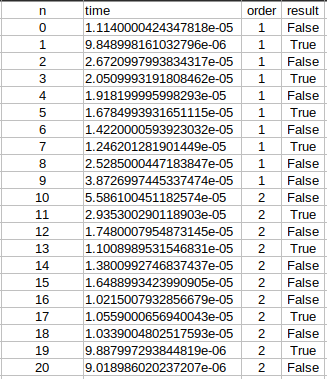
\includegraphics[width=5cm]{img/fucntional_test.png}}
\end{figure}
  